%% BioMed_Central_Tex_Template_v1.06
%%                                      %
%  bmc_article.tex            ver: 1.06 %
%                                       %

%%IMPORTANT: do not delete the first line of this template
%%It must be present to enable the BMC Submission system to 
%%recognise this template!! Receiving my "Resident Permit" to stay in Great Britain on the day when they decided to withdrew their residence from.. 

%%%%%%%%%%%%%%%%%%%%%%%%%%%%%%%%%%%%%%%%%
%%                                     %%
%%  LaTeX template for BioMed Central  %%
%%     journal article submissions     %%
%%                                     %%
%%         <14 August 2007>            %%
%%                                     %%
%%                                     %%
%% Uses:                               %%
%% cite.sty, url.sty, bmc_article.cls  %%
%% ifthen.sty. multicol.sty		   %%
%%				      	   %%
%%                                     %%
%%%%%%%%%%%%%%%%%%%%%%%%%%%%%%%%%%%%%%%%%


%%%%%%%%%%%%%%%%%%%%%%%%%%%%%%%%%%%%%%%%%%%%%%%%%%%%%%%%%%%%%%%%%%%%%
%%                                                                 %%	
%% For instructions on how to fill out this Tex template           %%
%% document please refer to Readme.pdf and the instructions for    %%
%% authors page on the biomed central website                      %%
%% http://www.biomedcentral.com/info/authors/                      %%
%%                                                                 %%
%% Please do not use \input{...} to include other tex files.       %%
%% Submit your LaTeX manuscript as one .tex document.              %%
%%                                                                 %%
%% All additional figures and files should be attached             %%
%% separately and not embedded in the \TeX\ document itself.       %%
%%                                                                 %%
%% BioMed Central currently use the MikTex distribution of         %%
%% TeX for Windows) of TeX and LaTeX.  This is available from      %%
%% http://www.miktex.org                                           %%
%%                                                                 %%
%%%%%%%%%%%%%%%%%%%%%%%%%%%%%%%%%%%%%%%%%%%%%%%%%%%%%%%%%%%%%%%%%%%%%


\NeedsTeXFormat{LaTeX2e}[1995/12/01]
\documentclass[10pt]{bmc_article}    



% Load packages
\usepackage{cite} % Make references as [1-4], not [1,2,3,4]
\usepackage{url}  % Formatting web addresses  
\usepackage{ifthen}  % Conditional 
\usepackage{multicol}   %Columns
\usepackage[utf8]{inputenc} %unicode support
\usepackage{graphicx}
%\usepackage[applemac]{inputenc} %applemac support if unicode package fails
%\usepackage[latin1]{inputenc} %UNIX support if unicode package fails
\urlstyle{rm}
\usepackage{placeins}
 
 
%%%%%%%%%%%%%%%%%%%%%%%%%%%%%%%%%%%%%%%%%%%%%%%%%	
%%                                             %%
%%  If you wish to display your graphics for   %%
%%  your own use using includegraphic or       %%
%%  includegraphics, then comment out the      %%
%%  following two lines of code.               %%   
%%  NB: These line *must* be included when     %%
%%  submitting to BMC.                         %% 
%%  All figure files must be submitted as      %%
%%  separate graphics through the BMC          %%
%%  submission process, not included in the    %% 
%%  submitted article.                         %% 
%%                                             %%
%%%%%%%%%%%%%%%%%%%%%%%%%%%%%%%%%%%%%%%%%%%%%%%%%                     


%\def\includegraphic{}
%\def\includegraphics{}



\setlength{\topmargin}{0.0cm}
\setlength{\textheight}{21.5cm}
\setlength{\oddsidemargin}{0cm} 
\setlength{\textwidth}{16.5cm}
\setlength{\columnsep}{0.6cm}

\newboolean{publ}

%%%%%%%%%%%%%%%%%%%%%%%%%%%%%%%%%%%%%%%%%%%%%%%%%%
%%                                              %%
%% You may change the following style settings  %%
%% Should you wish to format your article       %%
%% in a publication style for printing out and  %%
%% sharing with colleagues, but ensure that     %%
%% before submitting to BMC that the style is   %%
%% returned to the Review style setting.        %%
%%                                              %%
%%%%%%%%%%%%%%%%%%%%%%%%%%%%%%%%%%%%%%%%%%%%%%%%%%
 

%Review style settings
\newenvironment{bmcformat}{\begin{raggedright}\baselineskip20pt\sloppy\setboolean{publ}{false}}{\end{raggedright}\baselineskip20pt\sloppy}

%Publication style settings
%\newenvironment{bmcformat}{\fussy\setboolean{publ}{true}}{\fussy}



% Begin ...
\begin{document}
\begin{bmcformat}


%%%%%%%%%%%%%%%%%%%%%%%%%%%%%%%%%%%%%%%%%%%%%%
%%                                          %%
%% Enter the title of your article here     %%
%%                                          %%
%%%%%%%%%%%%%%%%%%%%%%%%%%%%%%%%%%%%%%%%%%%%%%

\title{Building blocks for automated elucidation of metabolites: Natural product-likeness for candidate ranking}
 
%%%%%%%%%%%%%%%%%%%%%%%%%%%%%%%%%%%%%%%%%%%%%%
%%                                          %%
%% Enter the authors here                   %%
%%                                          %%
%% Ensure \and is entered between all but   %%
%% the last two authors. This will be       %%
%% replaced by a comma in the final article %%
%%                                          %%
%% Ensure there are no trailing spaces at   %% 
%% the ends of the lines                    %%     	
%%                                          %%
%%%%%%%%%%%%%%%%%%%%%%%%%%%%%%%%%%%%%%%%%%%%%%


\author{Kalai Vanii Jayaseelan\correspondingauthor$^{1}$%
       \email{Kalai Vanii Jayaseelan\correspondingauthor - kalai@ebi.ac.uk}%
        \and
         Christoph Steinbeck\correspondingauthor$^{1}$%
         \email{Christoph Steinbeck\correspondingauthor - steinbeck@ebi.ac.uk}
      }
      

%%%%%%%%%%%%%%%%%%%%%%%%%%%%%%%%%%%%%%%%%%%%%%
%%                                          %%
%% Enter the authors' addresses here        %%
%%                                          %%
%%%%%%%%%%%%%%%%%%%%%%%%%%%%%%%%%%%%%%%%%%%%%%

\address{%
    \iid(1)Cheminformatics and Metabolism, European Molecular Biology Laboratory - European Bioinformatics Institute (EMBL-EBI), Wellcome Trust Genome Campus, Hinxton, Cambridge, CB10 1SD, UK.
  }%

\maketitle

%%%%%%%%%%%%%%%%%%%%%%%%%%%%%%%%%%%%%%%%%%%%%%
%%                                          %%
%% The Abstract begins here                 %%
%%                                          %%
%% The Section headings here are those for  %%
%% a Research article submitted to a        %%
%% BMC-Series journal.                      %%  
%%                                          %%
%% If your article is not of this type,     %%
%% then refer to the Instructions for       %%
%% authors on http://www.biomedcentral.com  %%
%% and change the section headings          %%
%% accordingly.                             %%   
%%                                          %%
%%%%%%%%%%%%%%%%%%%%%%%%%%%%%%%%%%%%%%%%%%%%%%


\begin{abstract} 
        % Do not use inserted blank lines (ie \\) until main body of text.
        \paragraph*{BACKGROUND:}
In metabolomics experiments, spectral fingerprints of metabolites with no known structural identity are routinely detected from the samples. Computer assisted structure elucidation (CASE) can be used to determine the structural identities of these unknown compounds in a fast and in more or less automated fashion. Provided a suite of spectra from 1D and 2D NMR experiments supplemented with molecular formula, successful elucidation of chemical structure for cases up to 30 heavy atoms have been previously reported by one of us. In high-throughput metabolomics usually 1D NMR experiments are conducted for rapid analysis of samples, which subsequently demand an automated analysis of the spectral patterns to quickly identify the knowns and the unknowns. The current scenario thus calls us to develop structure identification methods to identify unknowns with as little experimental input as possible. It is common knowledge and has been confirmed by our analysis that 1D NMR alone is usually not sufficient to establish the identity of a hitherto unknown compound. 
      \paragraph*{RESULTS:} 
       Towards an attempt to identify unknowns with as little spectroscopic information as possible, we have implemented an evolutionary algorithm based CASE mechanism that attempts to elucidate candidates in a fully automated fashion, with input of molecular formula and $^{13}C$ NMR spectrum of the isolated compound from the mixture. In addition, we have tested, how filters like natural product likeness - a measure that calculates the similarity of the compounds to known natural product space, enhance the performance and quality of the structure elucidation.
      The evolutionary approach is implemented within the already reported CASE system Seneca, and is available for free download under artistic license at \url{http://sourceforge.net/projects/seneca/}. The natural product-likeness calculator is incorporated as a plugin within Seneca. The tool is available both as a GUI client and command line executable. Significant improvement in candidate ranking when supplemented by natural product-likeness filter, is demonstrated for 41 test small molecules using the implemented CASE system.
        %%% standalone JAR yet to be uploaded

        \paragraph*{CONCLUSIONS:} In spectroscopically underdetermined structure elucidation problems, Natural Product Likeness can contribute to a better ranking of the correct structure in the results list.  
      
         \paragraph*{KEYWORDS:} Computer assisted structure elucidation, metabolomics, natural product likeness 
        \end{abstract}



\ifthenelse{\boolean{publ}}{\begin{multicols}{2}}{}



%%%%%%%%%%%%%%%%%%%%%%%%%%%%%%%%%%%%%%%%%%%%%%
%%                                          %%
%% The Main Body begins here                %%
%%                                          %%
%% The Section headings here are those for  %%
%% a Research article submitted to a        %%
%% BMC-Series journal.                      %%  
%%                                          %%
%% If your article is not of this type,     %%
%% then refer to the instructions for       %%
%% authors on:                              %%
%% http://www.biomedcentral.com/info/authors%%
%% and change the section headings          %%
%% accordingly.                             %% 
%%                                          %%
%% See the Results and Discussion section   %%
%% for details on how to create sub-sections%%
%%                                          %%
%% use \cite{...} to cite references        %%
%%  \cite{koon} and                         %%
%%  \cite{oreg,khar,zvai,xjon,schn,pond}    %%
%%  \nocite{smith,marg,hunn,advi,koha,mouse}%%
%%                                          %%
%%%%%%%%%%%%%%%%%%%%%%%%%%%%%%%%%%%%%%%%%%%%%%




%%%%%%%%%%%%%%%%
%% Background %%
%%
\section*{1. Background}

A significant amount of small molecules in the metabolism of organisms are still unknown. Methods for the structure elucidation of unknown metabolites are therefore needed. Computer-assisted structure elucidation (CASE) -- a field that has been researched for over 40 years \cite{Steinbeck:2001}, lends itself towards this end. For complex structure elucidation problems, a rich set of mass spectral as well as 1D and 2D NMR spectroscopic information is required \cite{steinbeck2003}. 

Under high-throughput conditions, however, only spectroscopic information that can be quickly recorded will be used. We are therefore investigating how successful structure determination can be, if only a limited set of spectroscopic information is available. While 1D proton NMR is the most commonly used NMR method in metabolomics, we are basing our study on carbon-13 NMR because reliable open source methods for proton prediction including coupling constants to produce realistic 1D spectra are not available. It is common knowledge and has been confirmed by our analysis that 1D NMR alone is usually not sufficient to establish the identity of a hitherto unknown compound.  We and others have recently demonstrated that metabolites and natural products cluster in a distinct area in structure space \cite{Peironcely:2011fm, Jayaseelan}. 

Here, we therefore would like show that natural product likeness can be used as another component to the fitness evaluators for our present effort to elucidate candidates with minimum spectral information and increase the likelihood of a natural product to rank highly in a resulting set of solutions. 
We have been implementing the methods presented here in our Seneca system, an open-source java based desktop application to perform CASE for organic molecules. The application takes molecular formula generated from high resolution mass spectrometry and spectral data from a suite of NMR experiments and performs stochastic search in the constitutional space, guided by a fitness function. With the above input, the ability of the application to elucidate correct structure for candidates up to 30 heavy atoms has been previously demonstrated. 

\section*{2. Methods}

The methods presented in this paper are implemented in the open source structure elucidation software Seneca 2.0. 
Seneca has been completely refactored  and is now based on the popular open-source cheminformatics library The Chemistry Development Kit (CDK) \cite{Luttmann,Guha}.   The CDK has graph-based, object-oriented representation of molecules and provides flexible functionalities to perform various operation on the molecule like valency check, ring perception, aromaticity detection, mutation, atom environment representation, to name a few. 
Seneca performs a stochastic search of constitution space (the space made up by all chemical compounds with the same gross formula), guided by a fitness or scoring function. This fitness function contains terms evaluating the similarity of predicted and experimental spectra as well as other terms evaluating the validity of the currently inspected solution. 
Seneca contains implementations of simulated annealing \cite{Steinbeck} and an evolutionary algorithm. The latter is a completely new implementation and not related to one previously reported \cite{Han} which was based on an older, obsolete library and therefore was discontinued.       
     
      
            \subsubsection*{Availability}
     The latest version of Seneca is available both as a desktop application and as a command-line executable. It is available for free download under artistic license at \url{http://sourceforge.net/projects/seneca/}.
   
	
\subsection*{2.1 Evolutionary algorithm for stochastic search}


 
 The EA technique is based on the Darwinian principles of evolution, incorporating the concepts of natural selection and survival of the fittest. The overall scheme implemented by us for our optimisation problem is similar to the one illustrated in \cite{Han}. The scheme reported in \cite{Han} has both mutation and recombination operators but we only decided to use the mutation operator as it offered the desired results. The simple EA scheme implemented by us is illustrated in \emph{figure} \ref{fig:EAprocedure}.
 
With our EA scheme, the evolution starts with a population of configurable number of randomly generated individuals, seeded by an initial molecular structure (connected graph) derived from the input molecular formula.  
To generate an initial population, the initial seed is randomly mutated by the mutation functionality within CDK based on the \emph{Faulon} mutation operator \cite{Faulon} . Each of the individual is evaluated for fitness by our fitness evaluators and cross checked with termination conditions. The program can be configured to terminate if any of the following criteria is reached: maximum fitness, maximum allowed runtime, maximum allowed generations, or maximum allowed generations with no improvement. For our purpose, we only used one termination condition - maximum allowed generations; in that way we could collect all isomers traversed, rank them and see if there is significant improvement in ranking of exact structure with the application  of NP-likeness filter. If the termination conditions are not met, each individual is mutated to generate one offspring, thereby doubling the population. The doubled population is evaluated for fitness again and the fittest individuals are chosen by round-robin tournament selection. If there is no improvement in fitness for five consecutive generations, fresh individuals are added to the population by doing vicinity search around the top two fittest individuals. After the niche search the population is expanded to size 24 from 16 and allowed to run for 5 generations. If again no fitness improvement is recorded the population size is reduced back to 16 using tournaments selection. The above evolution procedure is repeated until the termination conditions are met (default maximum allowed generations: 3000). Once met, the evolution is stopped and the elucidated candidates are reported. 

\subsection*{2.2 Fitness evaluators}
 
 A suite of fitness evaluators (judges), each evaluating a certain optimisation criterion, i.e. agreement between the recorded chemical shift value from various NMR techniques ($^{13}C$ NMR, HHCOSY, HMBC and HSQC) 
 and the observed structural features in the candidate, has been already presented in Seneca \cite{Steinbeck} and also refreshed in \cite{Han}. We are not going to discuss the scoring methods used by these judges in detail here, but discuss only the newly implemented fitness evaluators that has not been previously reported. 
 
 \subsection*{NMRShiftDB judge}
  NMRShiftDB is an open-source database that houses around 42,000 organic molecules associated with its recorded experimental 1D NMR spectra \cite{Kuhn}. The database has moved from its original host since his first publication and its new instance can be accessed at  \url{http://nmrshiftdb.nmr.uni-koeln.de/}. \texttt{HoseCodeJudge}, a fitness evaluator from older version of Seneca \cite{Steinbeck}, does simple back calculation of chemical shift by generating one sphere HOSE code \cite{Bremser:1977} for each Carbons in the candidate, and by looking them up individually in the table of 651 one-sphere  \emph{HOSE - $^{13}C$ shift} entries published by \emph{Bremser} \cite{Bremser:1985}. If the back-calculated and the experimental shift's absolute deviation is with in the confidence limit offered for that shift value, full points is awarded for that Carbon, and zero otherwise. The summation from all the Carbons give the total score, validating the agreement between the $^{13}C$ spectrum and the expected atom environments, also helping to keep the hybridisation and heteroatom attachments in check. 
  
 The precision of prediction by \texttt{HoseCodeJudge} can be improved if we can capture extended atom environment of the Carbons by increasing the HOSE sphere height \cite{Steinbeck}. So we decided to use NMRShiftDB database to produce an index of HOSE with extended heights (from 1 to 4) and associate it with a mean chemical shift and a confidence score, similar to  \emph{Bremser's} approach\cite{Bremser:1985}. To keep it simple, we decided not to include any intensity or multiplicity information in our index.
  
The mean shift value for each HOSE code, is calculated by averaging all the observed shifts over its molecule occurrence count. The standard deviation will therefore increase as the sphere height decreases. The confidence limit (CL) for each mean shift is calculated by multiplying the standard error with two-sided Student's t-distribution value for  95\% confidence.  If confidence limit is less than 5 ppm, a minimum value of  5 ppm is assigned.  The so generated index serves has a look up table for our new \texttt{NMRShiftDBJudge}. The judge calculates the $^{13}C$ spectrum ($\delta_{pred}$) for the candidate and gives it a fitness score based on its agreement with the experimental spectrum ($\delta_{exp}$) as shown in \emph{equation} \ref{eq : nmrscore}. If the absolute difference between the predicted and the experimental spectrum is less than CL, 100 points is given, else zero. For example a molecule with 10 Carbons, the total maximum \texttt{NMRShiftDBJudge} score will be 1000 and  \emph{equation} \ref{eq : nmrcost} can be applied to normalise the score between 0 and 1. 

   
  \begin{equation}
   Score_{nmr\_judge} = \sum_{Carbons} \Bigg\{
  \begin{array}{l l}
    100 & \quad \textrm{if $(\delta_{pred} - \delta_{exp})$ $<=$ CL} \\
    0 & \quad \textrm{if $(\delta_{pred} - \delta_{exp})$ $>$ CL}   
   \end{array} 
    \label{eq : nmrscore}
  \end{equation}
  
  
  
 
 \begin{equation}
NMRcost_{norm} = \frac{Score_{nmr\_judge}}{Carbon\_count * 100}
\label{eq : nmrcost}  
 \end{equation}
 
 
 
  
\subsection*{NPLikeness judge}

With only  \texttt{NMRShiftDBJudge} many isomers will emerge as the fittest by satisfying all the fragment to shift associations. This is a classic problem in CASE - the possibility of finding not one but many structural candidates satisfying the given NMR constraints. From these list of possibilities we need to then rely on expert opinion to pick a more or less correct candidate solution. Hence, candidate ranking methods are indispensable in CASE when there is numerous solution to a given problem.

One automated way to rank these candidate solutions is to check for their structural validity, for example, calculation of their structural similarity with that of known Natural Products (NPs).  Therefore, inclusion of a \texttt{NPLikenessJudge}, in such cases is expected to improve the ranking of the candidate solution by filtering out improbable structures on the fly during evolution. To make decisions on the NP-likeness of a molecule, knowledge about the structural space of known NPs as opposed to the synthetics is crucial. We have reported such a scorer based on the open-data of known natural products and synthetics \cite{Jayaseelan}, with the main motivation of including it in our CASE program. We have implemented a  \texttt{NPLikenessJudge} by including the NP-likeness calculator as a dependency within Seneca. The judge scores molecule for NP-likeness based on its degree of overlap with the known natural product space.
The NP score given is between -3.5 to + 3.5, where more positive the score, the more NP-like the molecule is and vice versa. We normalise this score between 0 to 1 by using the  \emph{equation} shown in \ref{eq : npcost}, where \emph{max} and \emph{min} are the extreme most values given by the NP-likeness scorer.


When \texttt{NPLikenessJudge} is used along \texttt{NMRShiftDBJudge} the total cost is calculated using the  \emph{equation} \ref{eq : totalcost}, by that way the molecule is weighted more for the NMR agreement and less for the NP-likeness. 

 \begin{equation}
NPcost_{norm} = \frac{Score_{np\_judge} - min} {max -min}
\label{eq : npcost}  
\end{equation}

 
 \begin{equation}
Cost_{total} = \Bigg[\frac{NMRcost_{norm}(1+NPcost_{norm})}{2}\Bigg]
\label{eq : totalcost}  
\end{equation}

 \subsection*{AntiBredt Judge}
 
 Another way to filter improbable structures during evolution is to check for structures that are sterically constrained. \texttt{AntiBredtJudge} penalises structure if it has double bond at bridge head atoms in rings of size seven or less. An implementation to detect these unrealistic structures has been previously reported \cite{Nuzillard} and we have re-used that logic in our CASE scheme. 
  

\subsection*{2.3 Test case collection}

In order to test the CASE system's performance in predicting the correct structures just with the $^{13}C$ spectrum, we collected 41 test cases from \emph{Journal of Natural products}. For our testing purposes, we took only molecules from recent articles that are with heavy atom count $<=$15. From each article the following information were extracted: Molecular formula (MF), $^{13}C$ chemical shifts,  DEPT 90 and DEPT 135 assignments based on the Hydrogens attached to the Carbons, and the molecular structure. The MF and spectrum information is manually entered into Seneca GUI client and saved as a .sml file. The .sml is a internal file format in Seneca based on XML. The molecular structure information is drawn using structure drawer and saved as a MDL mol file for cross checking at the end. All of the structures were cross checked with the NMRShiftDB index and made sure that none is  already present in the index. The collected test cases are illustrated in \emph{figure} \ref{fig:testcases}.

\section*{3. Performance results of the CASE system}

 
We have tested the performance of Seneca only using our new fitness evaluators mentioned above: \texttt{NMRShiftDBJudge}, \texttt{NPLikenessJudge}, and \texttt{AntiBredtJudge}. In order to test the enhancement in candidate ranking with the application of NP-likeness, we had two different runs for our 41 test cases. The first run (\emph {NMR\_only}), included only  \texttt{NMRShiftDBJudge} and \texttt{AntiBredtJudge} and the second run (\emph {NMR\_NP}) included all the three judges. The stochastic search does not always guarantee to find the global optimum in one run and its usual to collect results from several runs, combine and rank them out. For our testing, we therefore did 100 sequential runs for every test case, i.e. 4100 runs each for  \emph {NMR\_only} and \emph {NMR\_NP} evaluations. Each of these runs execute an evolution that terminates after 3000 generations and report all the elucidated candidates back.

The first thing we observed from these test runs, is that the frequency of retrieving the correct structure in the solution set is more with \emph {NMR\_NP} judges than with just the \emph {NMR\_only} judges. This is shown in \emph{figure} \ref{fig:retrieval}. Although the retrieval percentage is low, there is 9.1\% overall improvement in predicting the correct candidates with the application of \emph {NMR\_NP} judges. Correct structures were retrieved in the solution set for 36/41 cases, with the application of our fitness evaluators. The cases for which no correct solution was found are the ones numbered 2, 4, 22, 28, and 35 in \emph{figure} \ref{fig:testcases}. That aside, the most interesting question to ask here is, in how many of these retrieved cases the correct candidate is ranked 1 and how frequently is it done so ?. The results answering the above question is shown in \emph{figure} \ref{fig:rank1s}. As illustrated, 9/34 cases and 17/35 cases were ranked 1 using \emph {NMR\_only} and \emph {NMR\_NP}  judges respectively. Not only does more candidates are correctly ranked as best, but also the frequency of correct candidate being ranked as the best increases with the application of NPLikeness filter. If we look at the best rank from 100 runs for each test case in \emph{figure} \ref{fig:bestRank}, application of NP-likeness not only performs consistently well alongside the NMR judge but also improve ranks where possible, except for 2 cases where candidates show unusually poor best rank with the application of \emph{NMR\_NP} judges.

The worst rank given to the test cases from 100 runs shown in \emph{figure} \ref{fig:worstRank}, depicts how \emph{NMR\_NP} judges keep the average ranks low by not exceeding the rank over 5000 with the exception of 3 test cases. \emph{Figure} \ref{fig:overallScores} gives us an idea of overall rank distribution for all test cases across all runs, where there was a correct candidate retrieval. The empty indices in the \emph{figure}  \ref{fig:overallScores}  indicate that there was no retrieval for that test case. From all these overall ranks obtained with and without NPlikeness, by averaging out the rank distribution as shown in \emph{figure} \ref{fig:averageRank}, we can see how application of  NPlikeness filter on average tends to improve the candidate ranks. 



\section*{Summary}

We have presented an open source, open data CASE system to deduce the unknowns often encountered in metabolomics and in natural product chemistry, with minimum experimental data input. 
An evolutionary scheme is implemented within Seneca \cite{Steinbeck}, and is available for use via GUI client or as a standalone command line executable. Fitness evaluators based on $^{13}C$ NMR spectrum to structure associations in NMRShiftDB database \cite{Kuhn}, and natural product likeness score \cite{Jayaseelan}, is integrated within the evolutionary scheme. With our available open-data based fitness evaluators, we have successfully demonstrated the elucidation of correct structures for unknowns in 36/41 test cases, with rank 1 for 17/36 cases and shown significant improvement in overall prediction frequency and average ranking with the application of NP-Likeness filter. This CASE system can be used in metabolomics data analysis pipelines to automatically deduce the unknowns with less than 15 heavy atoms and to significantly reduce the candidates space for molecules with more than 15 heavy atoms, which can then be subjected to further filters based on the biochemistry and species information to home in on the exact chemical structure. The open-source, open-data implementation enables other researchers to contribute to or modify the package, and use their own training data for fitness evaluation once they become available.

    
%%%%%%%%%%%%%%%%%%%%%%%%%%%%%%%%
\section*{Competing interests}

The authors declare that they have no competing interests.

\section*{Authors' contributions}

CS conceived the idea of testing the NP-likeness role in CASE. KJ conducted the study, selected the data, implemented EA scheme and new fitness evaluators within Seneca and tested it. All authors contributed to the manuscript, read and approved it. 

%%%%%%%%%%%%%%%%%%%%%%%%%%%
\section*{Acknowledgements}

KJ thanks her colleagues from Cheminformatics and metabolism group at EBI for their active support and critical comments. All authors are especially thankful to the post doc in the group, Luis Filipe de Figueiredo, for helping with the initial refactoring of Seneca and its upload to Sourceforge. All authors are also very grateful to the open-source communities of CDK. This work was supported by the funds from the BBSRC.   \ifthenelse{\boolean{publ}}{\small}{}
  
%%%%%%%%%%%%%%%%%%%%%%%%%%%%%%%%%%%%%%%%%%%%%%%%%%%%%%%%%%%%%
%%                  The Bibliography                       %%
%%                                                         %%              
%%  Bmc_article.bst  will be used to                       %%
%%  create a .BBL file for submission, which includes      %%
%%  XML structured for BMC.                                %%
%%  After submission of the .TEX file,                     %%
%%  you will be prompted to submit your .BBL file.         %%
%%                                                         %%
%%                                                         %%
%%  Note that the displayed Bibliography will not          %% 
%%  necessarily be rendered by Latex exactly as specified  %%
%%  in the online Instructions for Authors.                %% 
%%                                                         %%
%%%%%%%%%%%%%%%%%%%%%%%%%%%%%%%%%%%%%%%%%%%%%%%%%%%%%%%%%%%%%


{\ifthenelse{\boolean{publ}}{\footnotesize}{\small}
 \bibliographystyle{bmc_article}  % Style BST file
  \bibliography{bmc_article} }     % Bibliography file (usually '*.bib' ) 

%%%%%%%%%%%

\ifthenelse{\boolean{publ}}{\end{multicols}}{}

%%%%%%%%%%%%%%%%%%%%%%%%%%%%%%%%%%%
%%                               %%
%% Figures                       %%
%%                               %%
%% NB: this is for captions and  %%
%% Titles. All graphics must be  %%
%% submitted separately and NOT  %%
%% included in the Tex document  %%
%%                               %%
%%%%%%%%%%%%%%%%%%%%%%%%%%%%%%%%%%%
%%
%% Do not use \listoffigures as most will included as separate files


\section*{Figures}

\begin{figure*}[hbt]
  \centering
  	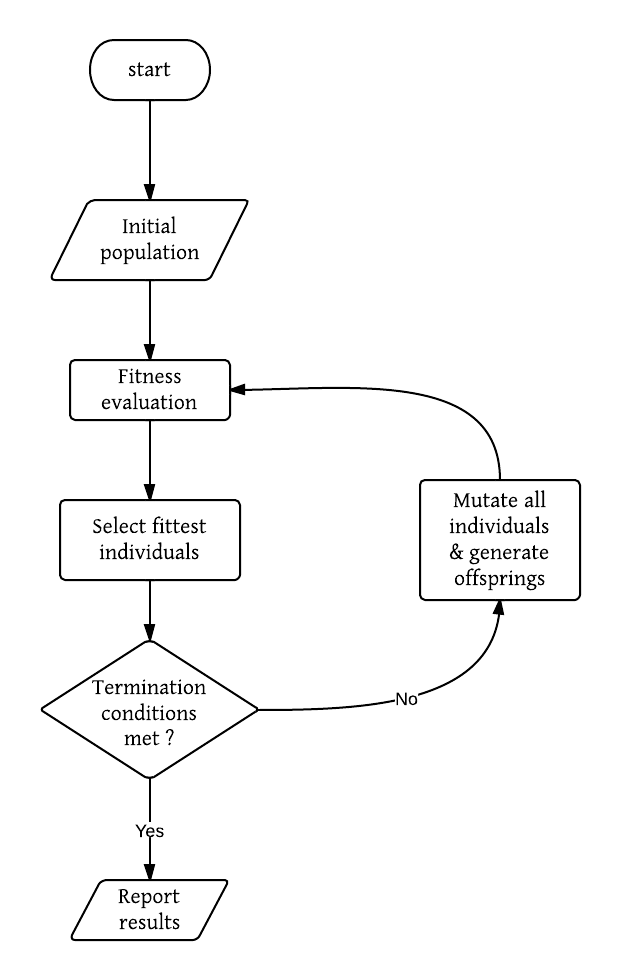
\includegraphics[angle=0,clip=false,scale=0.5]{pics/EAprocedure.png}
	
  \caption{Evolutionary algorithm scheme for CASE: The evolution starts with an initial population of 16 individuals. The initial population is seeded by mutating the single random structure generated from the molecular formula. The population is evaluated for termination criteria, i.e. either of the following: maximum fitness, maximum allowed runtime, maximum allowed generations, or maximum allowed generations with no improvement. Evolution continues until any of the above conditions are met. The population is doubled by mutating every individual before fitness is evaluated. After fitness evaluation, the fittest ones are promoted to the next generation by round-robin tournaments selection. Once the termination conditions are met, the solution set is reported.}
   
  \label{fig:EAprocedure}
\end{figure*}

\begin{figure*}[hbt]
  \centering
  	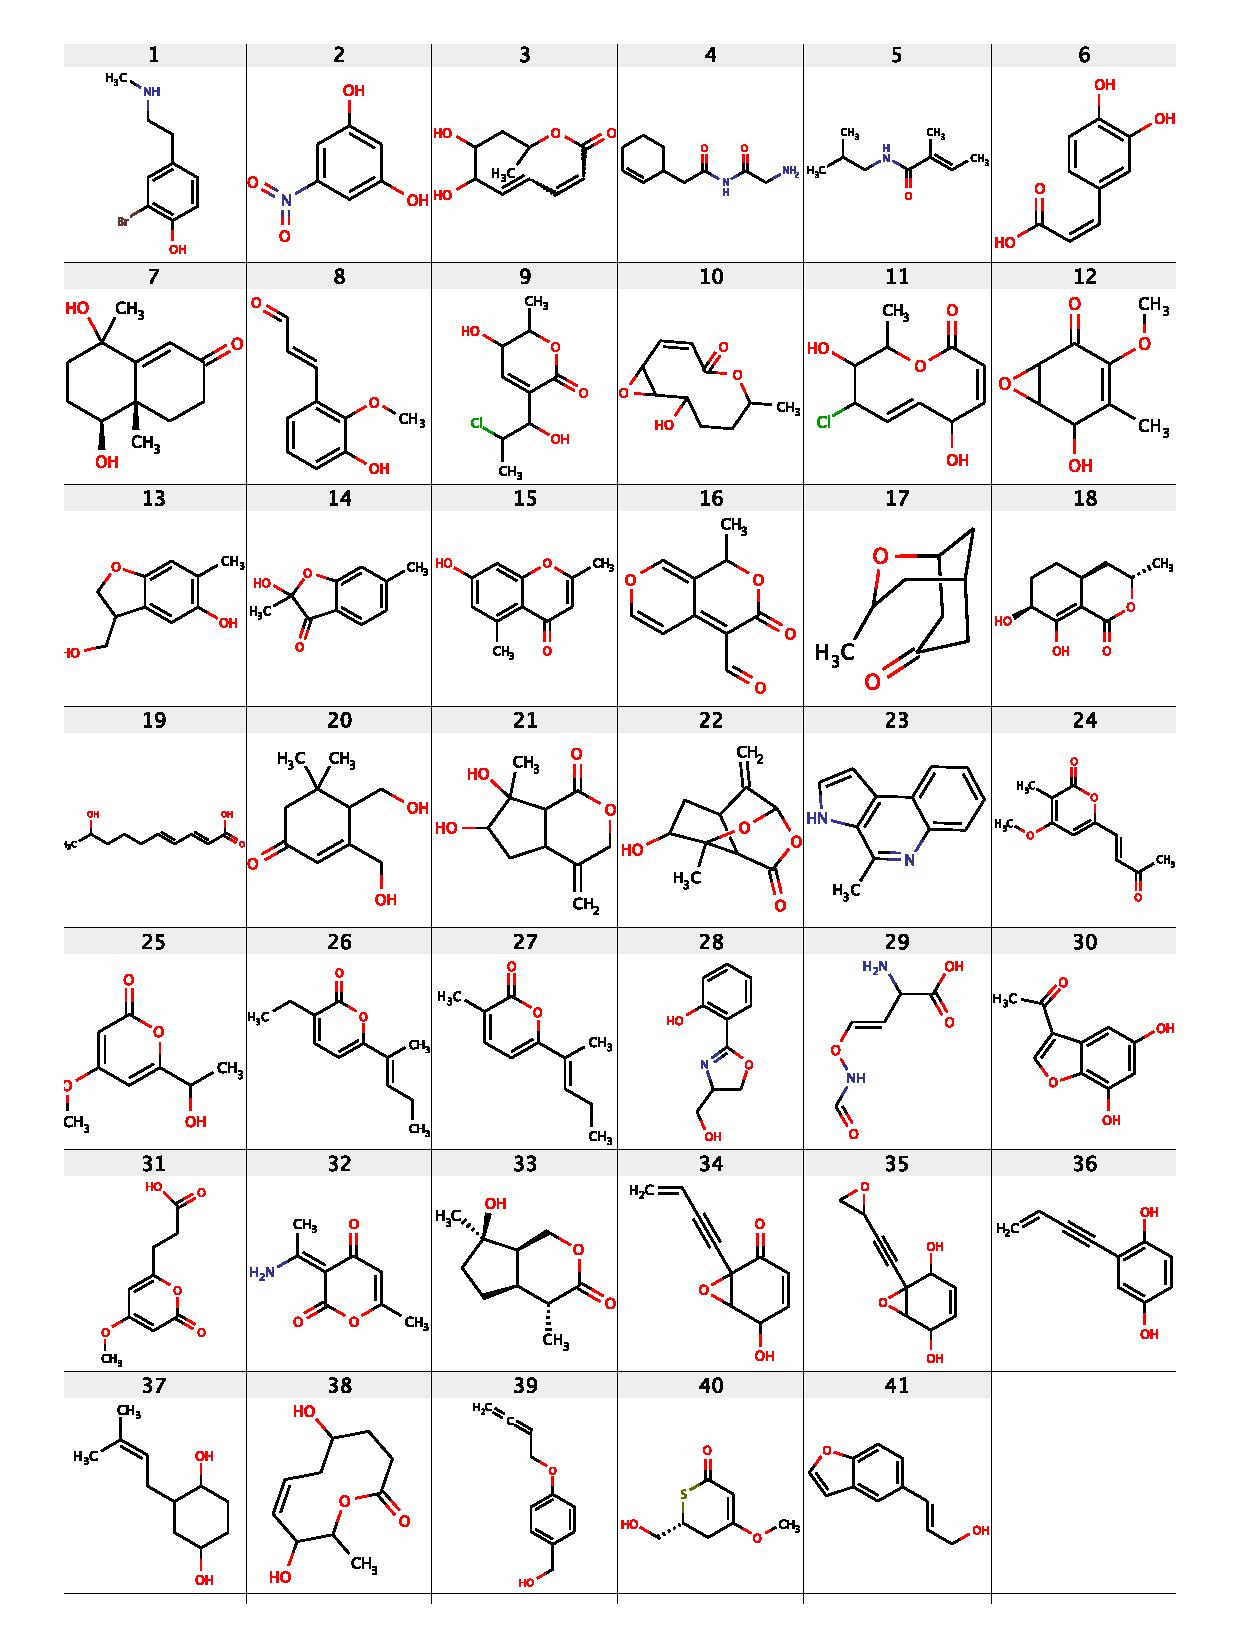
\includegraphics[angle=0,clip=false,scale=0.5]{pics/testcases.pdf}
	
  \caption{Test cases collected from \emph{Journal of natural products}: For our testing purposes, we took only molecules from recent articles that are with heavy atom count $<=$15. All of these structures were cross checked with the NMRShiftDB index and made sure that none is  already present in the index.}
   
  \label{fig:testcases}
\end{figure*}

\begin{figure*}[hbt]
  \centering
  	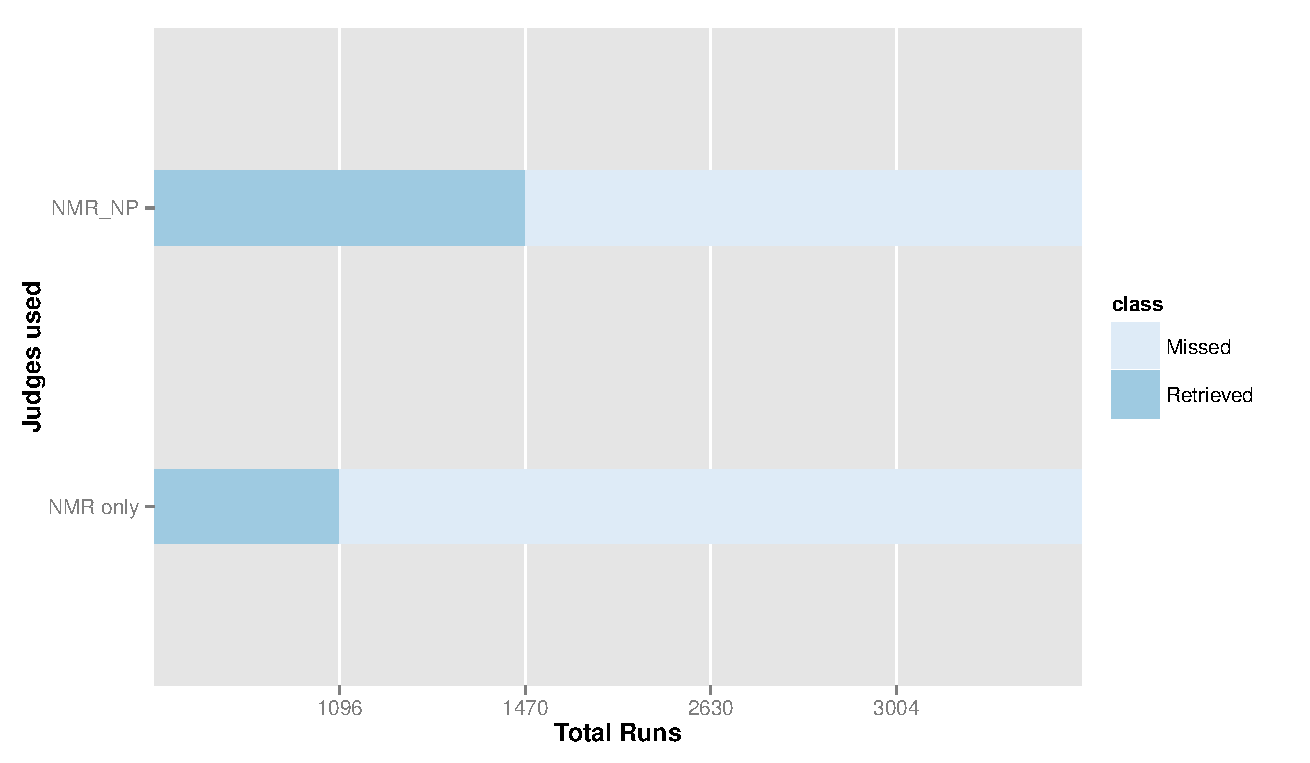
\includegraphics[angle=0,clip=false,scale=0.5]{pics/retrieval.pdf}
	
  \caption{NMR+NP judges retrieve correct solutions more often:  The stochastic search does not always guarantee to find the global optimum in one run and its usual to collect results from several runs, combine and rank them out. For our testing, we therefore did 100 sequential runs for every 41 test case, i.e. 4100 runs each for  \emph {NMR\_only} and \emph {NMR\_NP} evaluations.  Correct candidates were retrieved in the solution set in 1470/4100 runs, and 1096/4100 runs, using \emph {NMR\_NP} and \emph {NMR\_only}, respectively.}
   
  \label{fig:retrieval}
\end{figure*}

\begin{figure*}[hbt]
\centering
	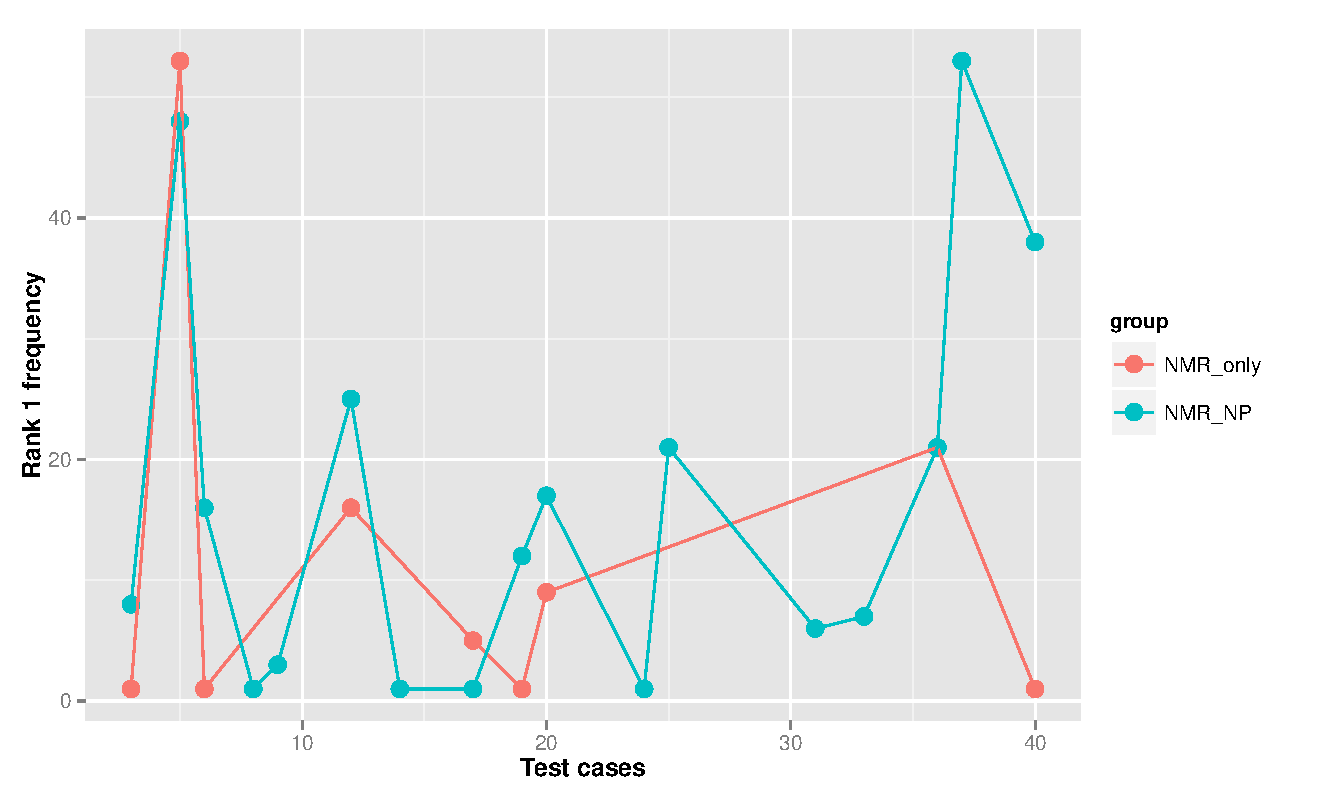
\includegraphics[angle=0,clip=false,scale=0.5]{pics/rank1s.pdf}
	\caption{Frequency of 1st ranks obtained by test cases using different judges: Correct structures were predicted for 36/41 test cases. Out of those correctly predicted ones, 9/34 cases and 17/35 cases were ranked 1 using \emph {NMR\_only} and \emph {NMR\_NP}  judges respectively. Not only does more candidates are correctly ranked as best, but also the frequency of correct candidate being ranked as the best increases with the application of NPLikeness filter.}
	\label{fig:rank1s}
\end{figure*}

\begin{figure*}[hbt]
  \centering
  	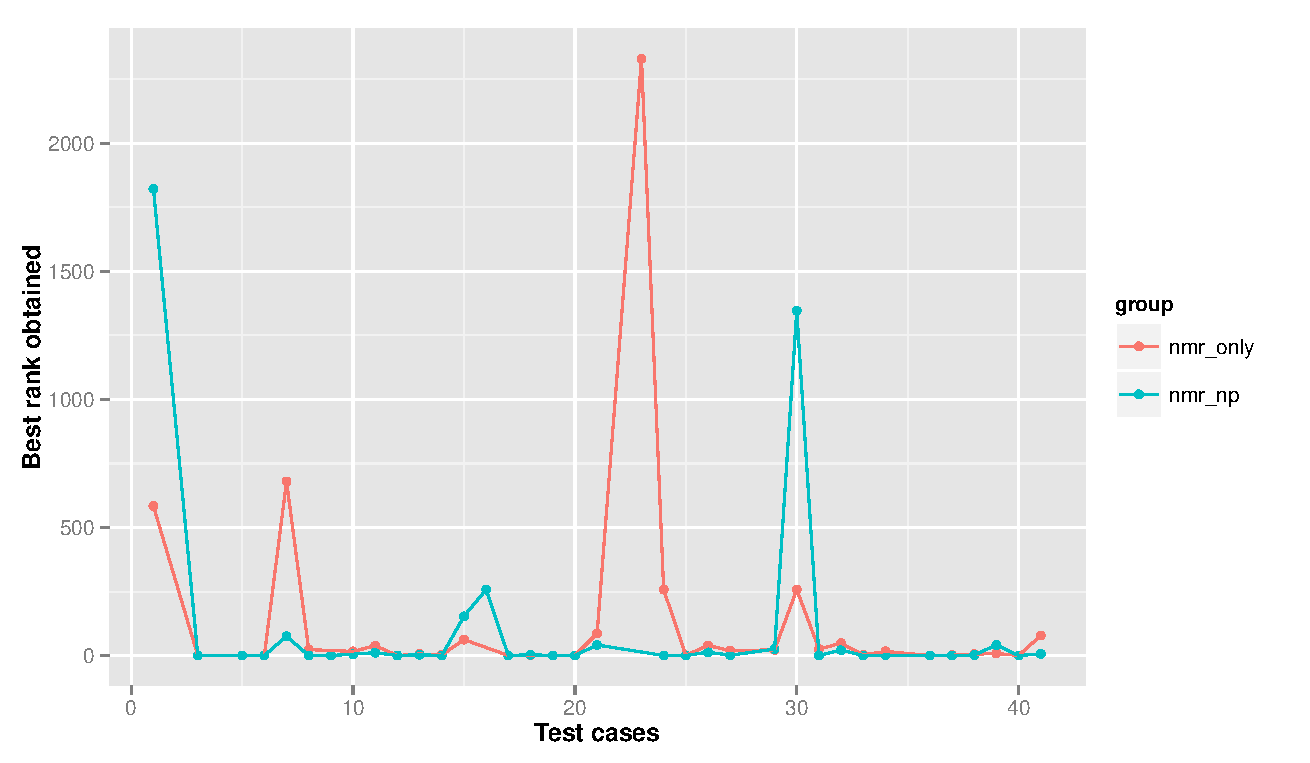
\includegraphics[angle=0,clip=false,scale=0.5]{pics/bestRank.pdf}	
  \caption{Best rank obtained in 100 different runs for every test case: Except for 2 cases where candidates show unusually poor best rank with the application of \emph{NMR\_NP} judges, overall application of NP-likeness not only performs consistently well alongside the NMR judge but also improves rank where possible and predicts structure where NMR only judge fail.}
   
  \label{fig:bestRank}
\end{figure*}

\begin{figure*}[hbt]
  \centering
  	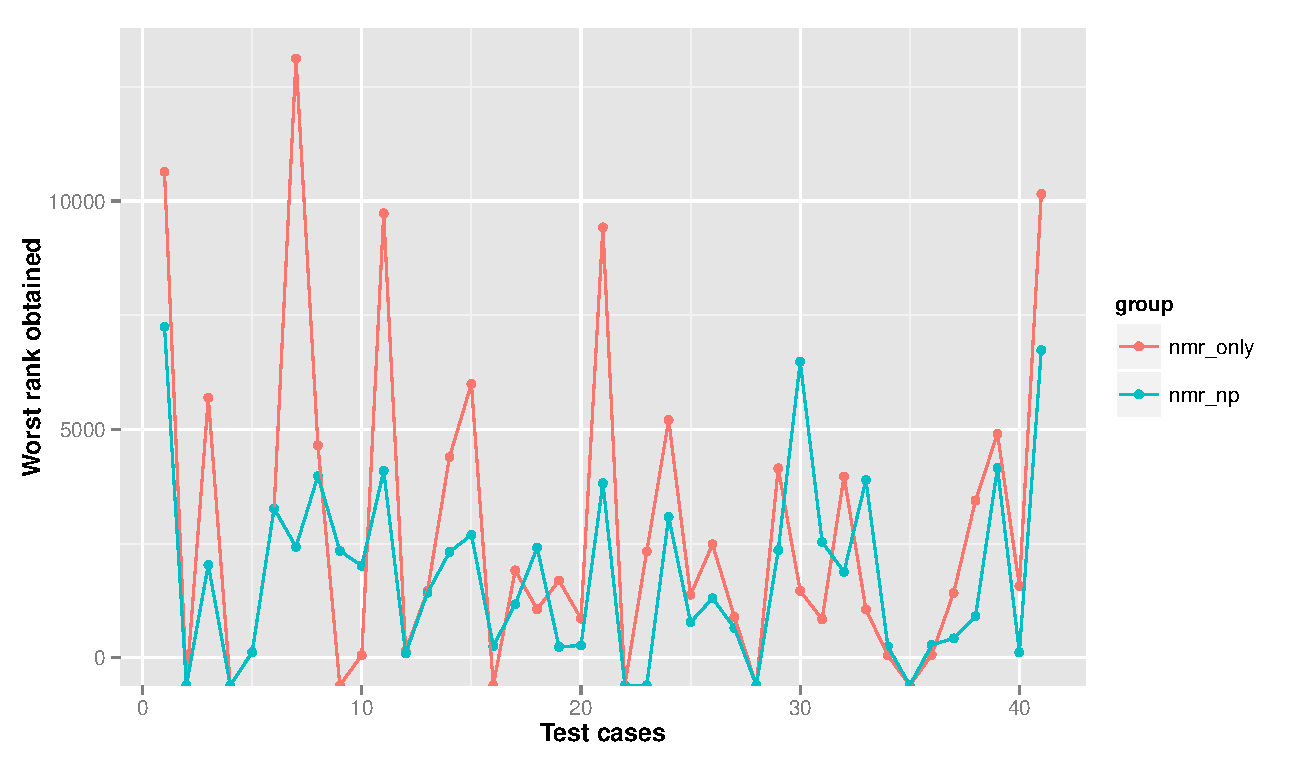
\includegraphics[angle=0,clip=false,scale=0.5]{pics/worstRank.pdf}
	
  \caption{Worst rank obtained in 100 different runs for every test case: With the exception of 3 test cases, the worst ranks depict how \emph{NMR\_NP} judges help keep the worst rank low by not exceeding the rank over 5000 when compared to the \emph{NMR\_only} judges.}
   
  \label{fig:worstRank}
\end{figure*}
\begin{figure*}[hbt]
  \centering
  	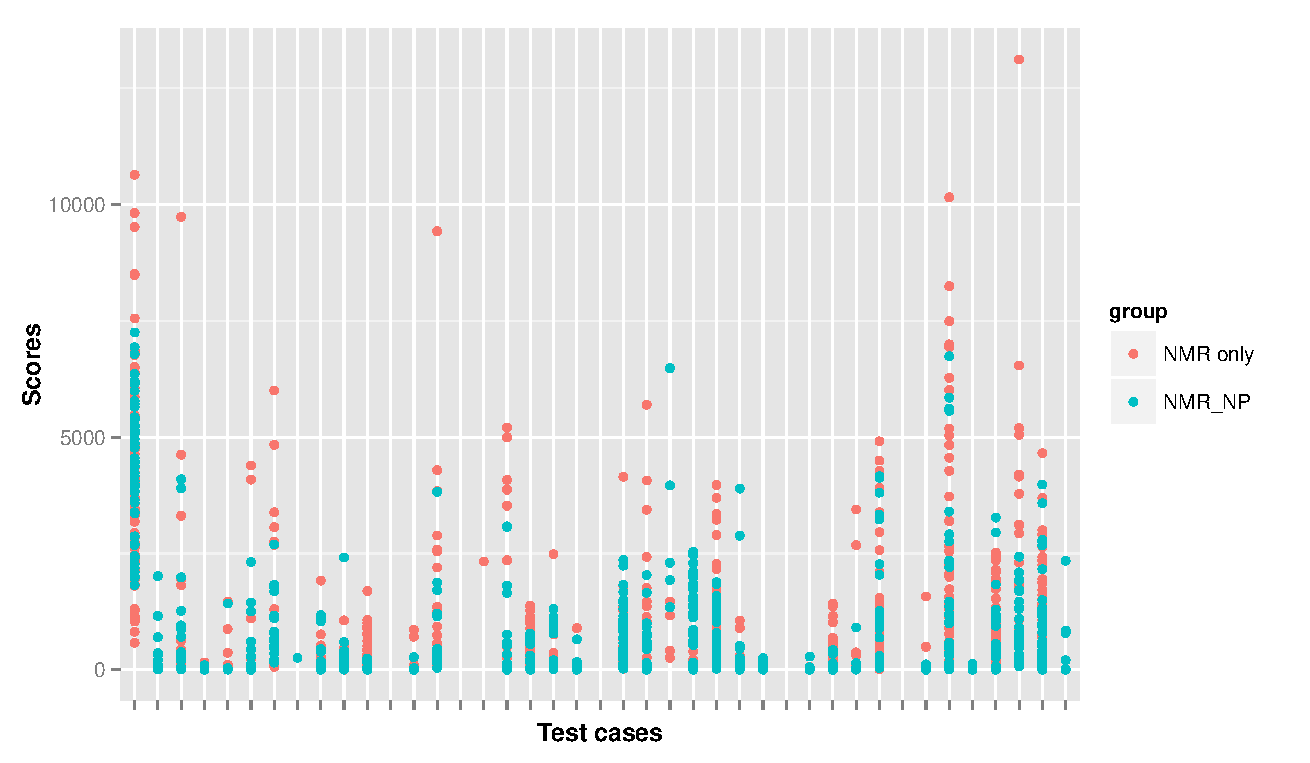
\includegraphics[angle=0,clip=false,scale=0.5]{pics/overallScores.pdf}
	
  \caption{Distribution of ranks across all test sets and runs:  The graph shows distribution of overall ranks given for all test cases, where there was a correct candidate retrieval across all runs. The empty indices indicate no retrieval for that test case.}
   
  \label{fig:overallScores}
\end{figure*}
\begin{figure*}[hbt]
  \centering
  	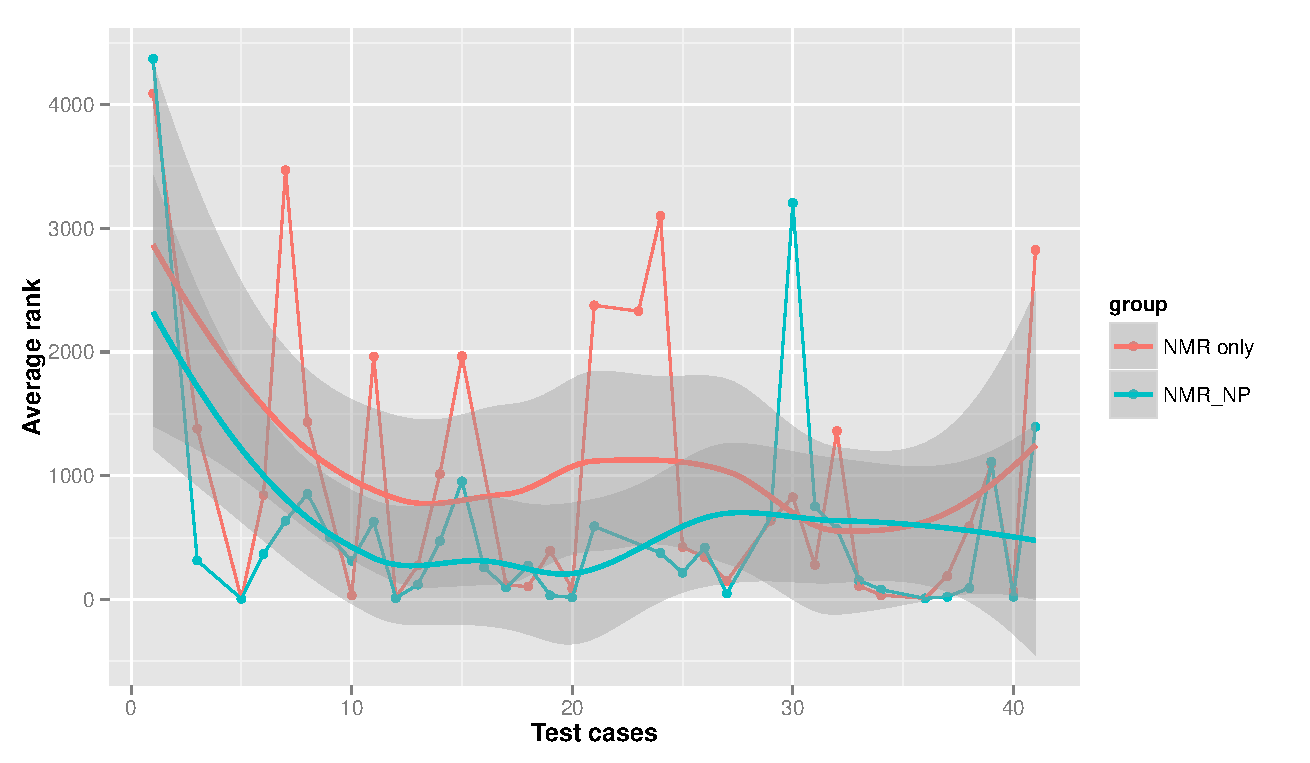
\includegraphics[angle=0,clip=false,scale=0.5]{pics/averageRank.pdf}
	
  \caption{Average rank obtained over 100 runs for each test case: The plot shows the averaged out rank from all the runs for every test case. Not only does application of NPlikeness predict correct candidates more often as shown in \emph{figure} \ref{fig:retrieval}, but also in all these retrievals on average improve the candidate ranks in comparison to the \emph{NMR\_only} judges. 
}
   
  \label{fig:averageRank}
\end{figure*}
   

   
\end{bmcformat}
\end{document}







